% =============================================================================
%  Report — Predicting the winner of a Counter-Strike 2 round
%  5 pages maximum (main body, appendices excluded)
%  Compile: pdflatex main.tex (x2)
% =============================================================================
\documentclass[11pt,a4paper]{article}

% ---- Encoding / language ----------------------------------------------------
\usepackage[utf8]{inputenc}
\usepackage[T1]{fontenc}
\usepackage[english]{babel}
\usepackage{lmodern}
\usepackage{microtype}
\usepackage{float}
\usepackage{placeins}

% ---- Layout -----------------------------------------------------------------
\usepackage[a4paper,margin=2cm]{geometry}
\usepackage{parskip}
\usepackage{setspace}
\setstretch{1.02}

% ---- Math / tables ----------------------------------------------------------
\usepackage{amsmath,amssymb}
\usepackage{booktabs}
\usepackage{array}

% ---- Listings (Python code, only used in the appendices) --------------------
\usepackage{listings}
\lstdefinestyle{pycode}{
  language=Python,
  basicstyle=\ttfamily\footnotesize,
  keywordstyle=\color{cs2ct}\bfseries,
  stringstyle=\color{cs2t!80!black},
  commentstyle=\color{gray}\itshape,
  showstringspaces=false,
  frame=single,
  rulecolor=\color{black!30},
  breaklines=true,
  numbers=left,
  numberstyle=\tiny\color{gray},
  numbersep=6pt,
}
\lstset{style=pycode}

% ---- Graphics / colors ------------------------------------------------------
\usepackage{graphicx}
\graphicspath{{figures/}}
\usepackage{xcolor}
\usepackage{tikz}
\usetikzlibrary{positioning,arrows.meta,shapes.geometric,fit,backgrounds}

\definecolor{cs2t}{HTML}{E8A020}
\definecolor{cs2ct}{HTML}{1E3A6E}

% ---- Hyperlinks -------------------------------------------------------------
\usepackage[colorlinks=true,linkcolor=cs2ct,citecolor=cs2ct,urlcolor=cs2t]{hyperref}

% ---- Section titles ---------------------------------------------------------
\usepackage{titlesec}
\titleformat{\section}
  {\color{cs2ct}\normalfont\large\bfseries}{\thesection}{0.7em}{}
\titlespacing*{\section}{0pt}{8pt}{4pt}
\titleformat{\subsection}
  {\color{cs2ct!90!black}\normalfont\normalsize\bfseries}{\thesubsection}{0.6em}{}
\titlespacing*{\subsection}{0pt}{6pt}{2pt}

% ---- Compact custom title block ---------------------------------------------
\makeatletter
\renewcommand{\maketitle}{%
  \begin{center}
    {\color{cs2ct}\Large\bfseries Predicting the winner of a Counter-Strike~2 round}\\[2pt]
    {\color{cs2ct}\normalsize Exploratory data analysis, PCA and logistic regression on a dataset of professional matches}\\[6pt]
    {\small Lucas Lacharme \;\textbullet\; \@date}
  \end{center}
}
\makeatother
\title{}
\author{}
\date{\today}

% =============================================================================
\begin{document}
% =============================================================================
\maketitle

\begin{abstract}
\noindent\small
Counter-Strike~2 is a 5-on-5 tactical shooter in which a team's
economy and overall skill level largely determine the outcome of each
round. From a dataset of \textbf{1{,}511 professional matches} and
\textbf{${\sim}32{,}000$ rounds} (Tier~1 tournaments, 2025--2026)
built by combining HLTV scraping with parsing of official demos, we
study how predictable the round winner is from the game state observed
just before the round begins (equipment, money, score, momentum).
Three regimes (\texttt{pistol}, \texttt{post-pistol}, \texttt{normal})
are analysed separately through correlation, PCA and logistic
regression.
\end{abstract}

% =============================================================================
%  Section 1 — Motivation
% =============================================================================
\section{Motivation}
\label{sec:motivation}

Counter-Strike~2 (\emph{CS2}) pits a team of
\textit{Counter-Terrorists} (\textcolor{cs2ct}{CT}) against a team of
\textit{Terrorists} (\textcolor{cs2t}{T}) over 24 rounds (MR12 format,
first team to 13 round wins). The T side tries to plant a bomb on one
of two sites; the CT side either prevents the plant or defuses the
bomb once it is down. Sides are swapped at half-time. Before each
round, a \emph{freeze-time} phase lets players buy weapons, armour and
grenades under an economic system whose payouts depend on previous
rounds. This rule set produces an asymmetry from one round to the next
and makes the \emph{game state measured right before the round begins}
potentially very informative about its outcome.

The central question is therefore:

\begin{center}\itshape\small
``Knowing the game state (equipment, money, score, momentum, rating
and recent form) at the instant a round starts, can we predict which
team is going to win that round?''
\end{center}

% =============================================================================

% =============================================================================
%  Section 2 — Data collection
% =============================================================================
\section{Data collection}
\label{sec:data}

No public source provides, for CS2, a round-level dataset aligned with
HLTV team statistics. We therefore build it by combining two streams:
the \emph{demos} (official replays downloaded from HLTV) from which we
extract, \textbf{round by round}, information about the game state at
the start of the round (equipment, money, weapon and utility counts,
etc.), and the \emph{team statistics} scraped from HLTV.org (rating,
ADR, round-win~\%, flash-assists, etc., broken down by map, side,
time window 30\,d/90\,d/6\,months and opponent tier). Figure
\ref{fig:pipeline} summarises the pipeline; the technical details
(snapshot tick, cleaning steps, NaN handling) are reported in
appendices A to C.

\begin{figure}[H]
\centering
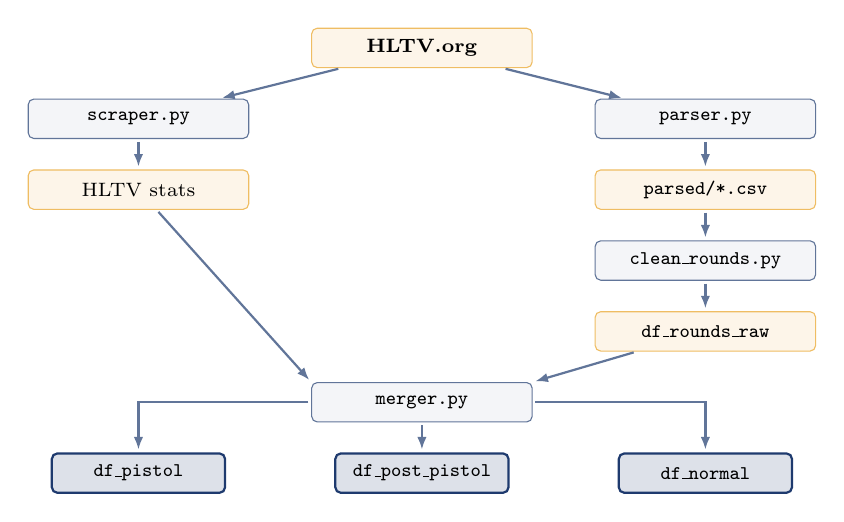
\begin{tikzpicture}[
  font=\scriptsize,
  >={Latex[length=1.6mm]},
  code/.style={draw=cs2ct!70, fill=cs2ct!5, rounded corners=2pt,
               minimum height=5mm, minimum width=28mm, align=center,
               inner sep=1.5pt},
  data/.style={draw=cs2t!70, fill=cs2t!10, rounded corners=2pt,
               minimum height=5mm, minimum width=28mm, align=center,
               inner sep=1.5pt},
  final/.style={draw=cs2ct, fill=cs2ct!15, rounded corners=2pt,
                thick, minimum height=5mm, minimum width=22mm, align=center,
                inner sep=1.5pt},
  arr/.style={->, thick, cs2ct!70, shorten >=1pt, shorten <=1pt},
]
\node[data] (hltv)    at ( 0,    0)    {\textbf{HLTV.org}};
\node[code] (scrap)   at (-3.6, -0.9)  {\texttt{scraper.py}};
\node[code] (parser)  at ( 3.6, -0.9)  {\texttt{parser.py}};
\node[data] (stats)   at (-3.6, -1.8)  {HLTV stats};
\node[data] (parsed)  at ( 3.6, -1.8)  {\texttt{parsed/*.csv}};
\node[code] (clean)   at ( 3.6, -2.7)  {\texttt{clean\_rounds.py}};
\node[data] (raw)     at ( 3.6, -3.6)  {\texttt{df\_rounds\_raw}};
\node[code] (merger)  at ( 0,   -4.5)  {\texttt{merger.py}};
\node[final] (pistol) at (-3.6, -5.4)  {\texttt{df\_pistol}};
\node[final] (postp)  at ( 0,   -5.4)  {\texttt{df\_post\_pistol}};
\node[final] (normal) at ( 3.6, -5.4)  {\texttt{df\_normal}};
\draw[arr] (hltv)  -- (scrap);
\draw[arr] (scrap) -- (stats);
\draw[arr] (hltv)  -- (parser);
\draw[arr] (parser) -- (parsed);
\draw[arr] (parsed) -- (clean);
\draw[arr] (clean)  -- (raw);
\draw[arr] (stats) -- (merger.north west);
\draw[arr] (raw)   -- (merger.north east);
\draw[arr] (merger) -| (pistol);
\draw[arr] (merger) -- (postp);
\draw[arr] (merger) -| (normal);
\end{tikzpicture}
\caption{Data collection pipeline.}
\label{fig:pipeline}
\end{figure}

\vspace{-0.6em}

\paragraph{Variables produced.}
Table~\ref{tab:features} groups the variables available after the
join by family: \emph{demo} variables are duplicated per side
(\texttt{ct\_*}, \texttt{t\_*}) and \emph{HLTV} statistics provide
18 to 24 indicators per team depending on the split. The target is
\texttt{round\_winner} ($1$ if CT wins, $0$ otherwise).

\begin{table}[H]
\centering
\footnotesize
\begin{tabular}{@{}lp{10.5cm}@{}}
\toprule
\textbf{Family} & \textbf{Main variables} \\
\midrule
Economy     & \texttt{money\_total}, \texttt{cash}, \texttt{equipment\_value},
              \texttt{utility\_value}, \texttt{loss\_count} \\
Weapons     & \texttt{awp\_count}, \texttt{rifle\_count}, \texttt{smg\_count},
              \texttt{heavy\_count}, \texttt{ak\_count} (T) \\
Armour      & \texttt{armor\_count}, \texttt{helmet\_count},
              \texttt{defuser\_count} (CT) \\
Utility     & \texttt{smoke\_count}, \texttt{flash\_count},
              \texttt{he\_count}, \texttt{molo\_count} \\
Context     & \texttt{round\_number}, \texttt{score},
              \texttt{survivors\_previous}, \texttt{previous\_bomb\_planted} \\
Momentum    & \texttt{rounds\_won\_streak}, \texttt{rounds\_lost\_streak} \\
HLTV stats  & rating, ADR, round-win\,\%, flash-assists, etc., broken
              down by map, side, time window and opponent tier \\
Identifiers & \texttt{match\_file}, \texttt{map\_name}, \texttt{match\_date},
              \texttt{round\_winner} (target) \\
\bottomrule
\end{tabular}
\caption{Variable families after the join.}
\label{tab:features}
\end{table}

% =============================================================================
%  Section 3 — Three round regimes + Pearson correlations
% =============================================================================
\section{Three round regimes}
\label{sec:split_pearson}

CS2 rounds are not equivalent. \textbf{Pistol rounds} (R1, R13) start
from an economy reset to \$800 per player: money and weapon variables
are nearly constant. \textbf{Post-pistol rounds} (R2, R14) display a
structural economic asymmetry caused by the pistol outcome (winner on
a \emph{full-buy}, loser on \emph{eco/force-buy}). \textbf{Normal
rounds} cover the rest of the game, where each team freely chooses
its buy depending on accumulated cash, and where all buy types (eco,
half-buy, force-buy, full-buy) coexist. Training a single model on
these three regimes would mix three very different distributions; we
therefore separate the dataset into three splits at join time
(Table~\ref{tab:splits}). All subsequent analysis (correlations, PCA,
regression) is carried out separately on each split.

\begin{table}[H]
\centering
\small
\begin{tabular}{lrrr}
\toprule
\textbf{Split} & \textbf{Rounds} & \textbf{Columns} & \textbf{CT win rate} \\
\midrule
\texttt{df\_pistol}       & $2{,}945$  & 70  & 50.5~\% \\
\texttt{df\_post\_pistol} & $2{,}956$  & 105 & 52.3~\% \\
\texttt{df\_normal}       & $26{,}322$ & 106 & 51.1~\% \\
\bottomrule
\end{tabular}
\caption{Final partition of rounds.}
\label{tab:splits}
\end{table}

\subsection{Pearson correlations with \texttt{round\_winner}}
\label{subsec:pearson}

Our target is \texttt{round\_winner}, coded $Y = 1$ if CT wins the
round and $Y = 0$ otherwise. To quickly assess the strength of the
linear link between each feature $X$ and $Y$, we use the Pearson
correlation coefficient, bounded in $[-1, +1]$:
\[
r_{X,Y} = \frac{\operatorname{cov}(X,Y)}{\sigma_X\,\sigma_Y}
        = \frac{\sum_{i=1}^{n}(x_i-\bar x)(y_i-\bar y)}
               {\sqrt{\sum_{i=1}^{n}(x_i-\bar x)^2}\,\sqrt{\sum_{i=1}^{n}(y_i-\bar y)^2}}.
\]
For each round we form the \emph{deltas}
$\Delta X = X^{\text{CT}} - X^{\text{T}}$ of the economic and HLTV
features, and we compute $r$ between each $\Delta X$ and $Y$ on each
of the three splits (Figure~\ref{fig:correlations}).

Profiles are very contrasted. In \textbf{pistol} rounds all
correlations stay below $|r| < 0.06$: no individual feature
discriminates strongly. In \textbf{post-pistol} rounds the economic
deltas (\texttt{equipment\_value}, \texttt{money\_total},
\texttt{utility\_value}, weapon counts) reach $|r| \approx 0.6$, a
direct signature of the asymmetry created by the pistol outcome. In
\textbf{normal} rounds the same deltas remain at the top but with a
more moderate amplitude ($|r| \approx 0.3$). Across all three regimes
we observe a clear separation between the two feature families:
parser-derived economic variables carry most of the signal while
HLTV statistics (rating, ADR, round-win~\%, \ldots) remain
systematically at a lower correlation level.

\begin{figure}[!t]
\centering
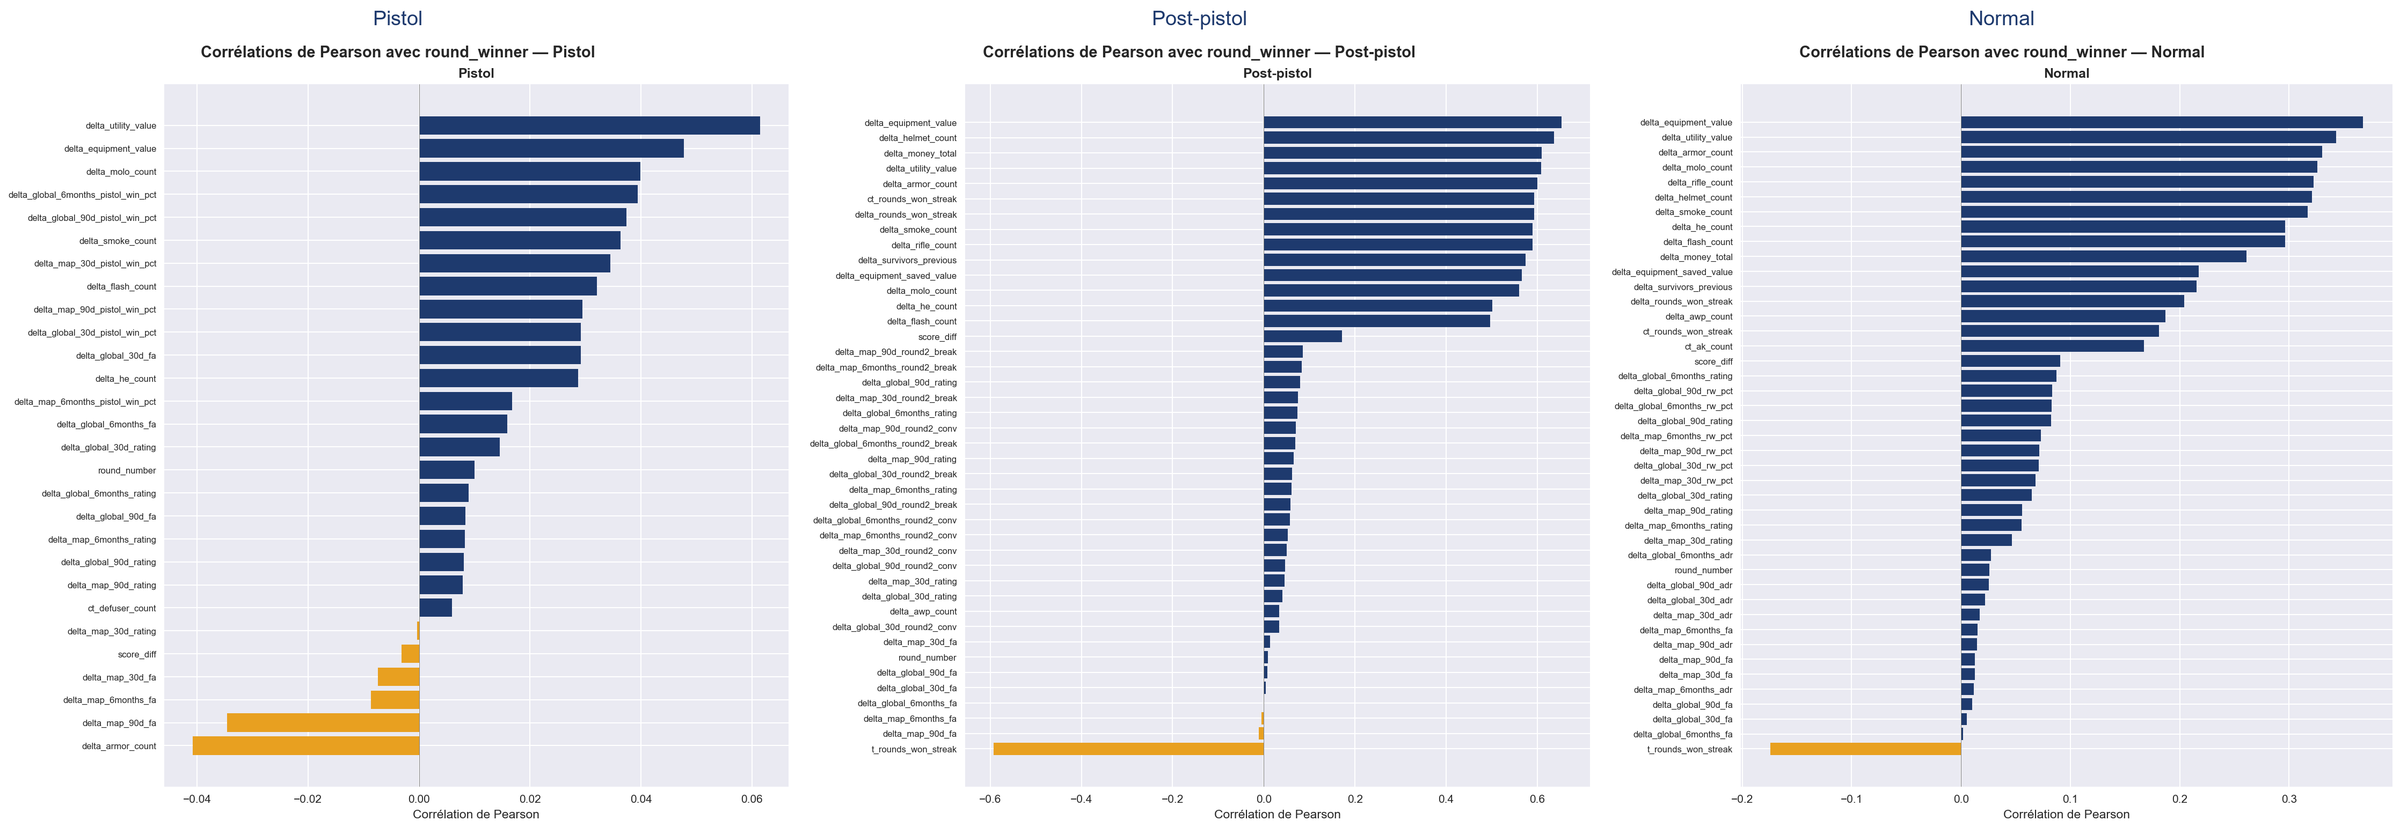
\includegraphics[width=\linewidth]{report_pearson_combined.png}
\caption{Pearson correlations between each CT~$-$~T delta and
\texttt{round\_winner}, by regime. Blue: positive correlation
(feature pushes toward a CT win); orange: negative.}
\label{fig:correlations}
\end{figure}

% =============================================================================

% =============================================================================
%  Section 4 — Analysis per regime
% =============================================================================
\section{Analysis per regime}
\label{sec:regimes}

\subsection{Pistol}
\label{subsec:pistol}

\begin{figure}[H]
\centering
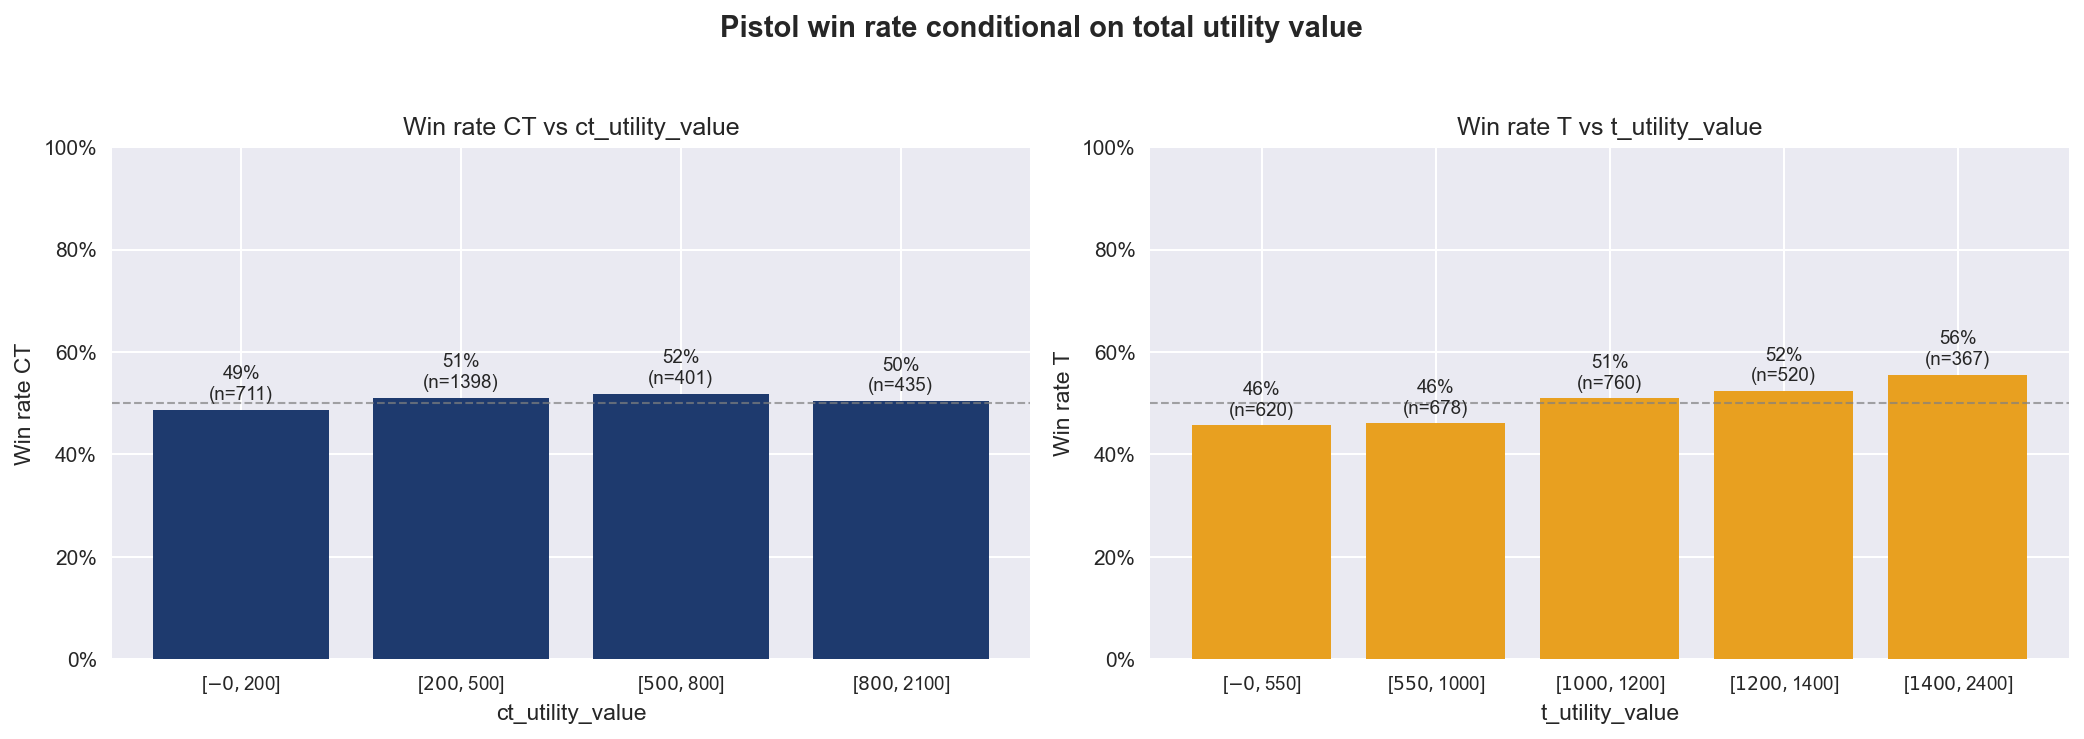
\includegraphics[width=\linewidth]{pistol_utility_winrate.png}
\caption{Pistol win rate conditional on the total
\texttt{utility\_value} purchased by the team, per quintile.}
\label{fig:pistol_utility}
\end{figure}

In pistol rounds, budgets are nearly equal and tightly bounded
(\$800/player), so very few features discriminate: all correlations
stay below $|r| < 0.06$. The only individual lever worth exploiting
is the \textbf{armour $\leftrightarrow$ utility} trade-off on the T
side, where skipping kevlar (\$650) to fund utility raises the win
rate by about 10 points (Figure~\ref{fig:pistol_utility}). The
\textbf{map} contributes a signal of comparable amplitude
(${\sim}8$~points between \texttt{de\_dust2} and \texttt{de\_anubis}).
HLTV statistics remain uninformative: the historical form of a team
does not transfer to pistol rounds, which behave almost like a coin
flip.

\subsection{Post-pistol}
\label{subsec:postpistol}

\begin{figure}[H]
\centering
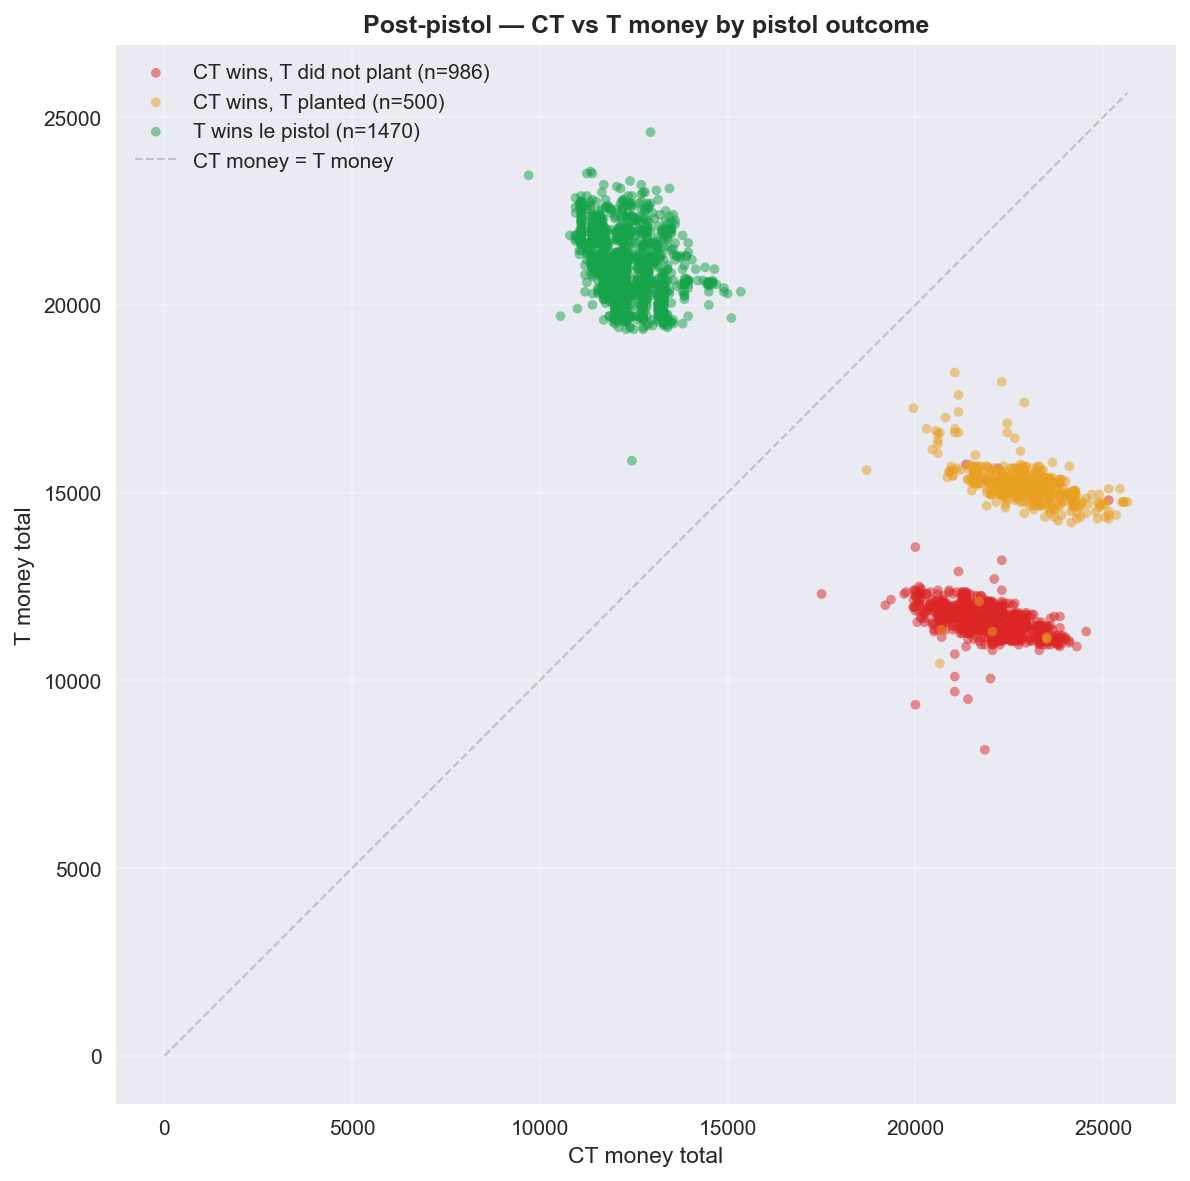
\includegraphics[width=0.45\linewidth]{post_pistol_money_scatter.png}
\caption{Post-pistol: CT \texttt{money\_total} vs T
\texttt{money\_total}, coloured by pistol outcome. The asymmetry is
sharp — pistol winner $\approx$ full buy, pistol loser $\approx$
eco/force.}
\label{fig:postpistol_money}
\end{figure}

The pistol outcome creates a structural \textbf{economic asymmetry}
between the winning team, which full-buys, and the losing team, whose
limited cash only allows an eco or a force-buy
(Figure~\ref{fig:postpistol_money}). This asymmetry translates into
\textbf{contrasted buy decisions} on the losing side: a near-systematic
force-buy on the CT side after a lost pistol (78~\%), versus only
48~\% on the T side. The T decision is actually conditioned by the
\emph{plant} of the bomb in the previous round. Its effect is directly
measurable on the force-buy profitability: without a plant the T
force-buy wins 26~\% of the time; with a plant the $+\$600$ per
player bonus is enough to lift it to 41~\%. This chain
\emph{asymmetry $\rightarrow$ decision $\rightarrow$ outcome} gives
post-pistol its exploitable signal, strongly correlated with the
pistol outcome.

\subsection{Normal}
\label{subsec:normal}

\begin{figure}[H]
\centering
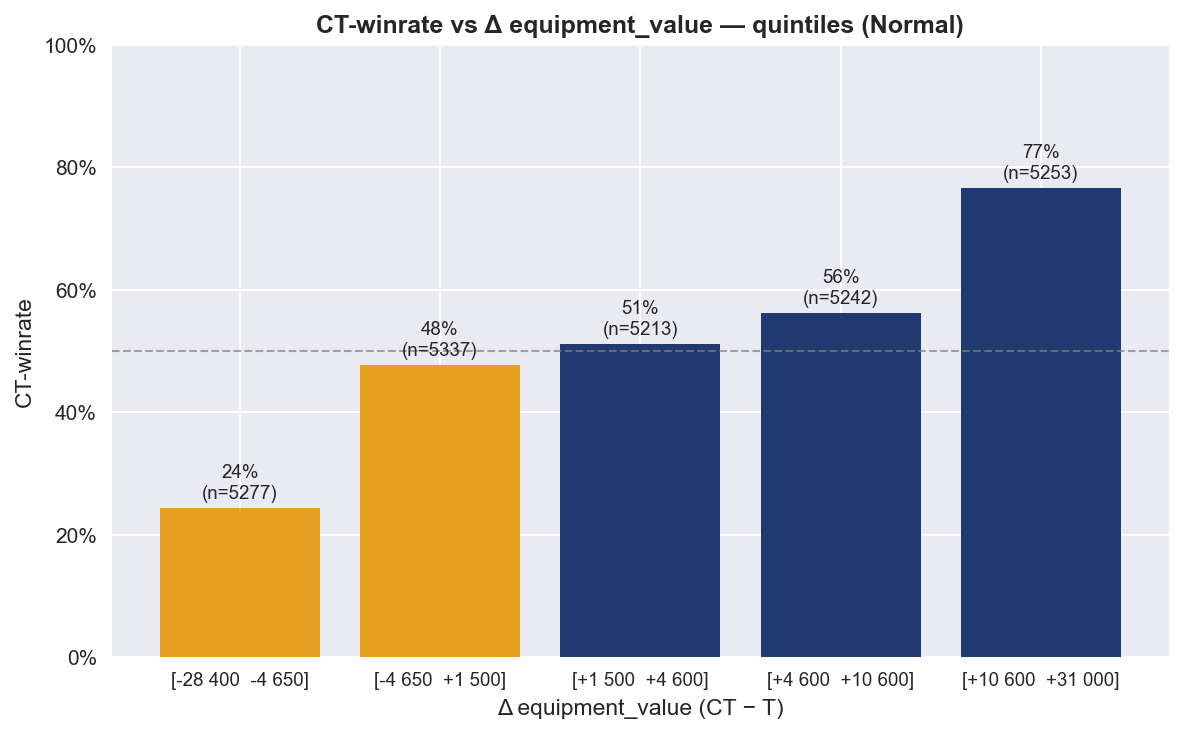
\includegraphics[width=0.6\linewidth]{normal_delta_eco_winrate.png}
\caption{CT win rate on normal rounds conditional on $\Delta$
\texttt{equipment\_value} (CT $-$ T), per quintile.}
\label{fig:normal_delta_equip}
\end{figure}

On normal rounds, all buy types coexist (eco, half-buy, force-buy,
full-buy) and the dominant signal is the economic gap measured
directly by $\Delta$ \texttt{equipment\_value}: its lowest quintile
corresponds to a win rate around 24~\% and its top quintile to 77~\%
(Figure~\ref{fig:normal_delta_equip}). At comparable economy (mutual
full-buy with \texttt{equipment\_value} $>$ 20\,k on both sides), two
secondary signals remain. The $\Delta$ \texttt{awp\_count} adds about
5 points of win rate per extra AWP; the map-specific HLTV rating
still separates teams but with a moderate amplitude (win rate
bounded in $[47\,\%, 55\,\%]$ between extreme quintiles).

% =============================================================================

% =============================================================================
%  Section 5 — PCA + Logistic Regression
% =============================================================================
\section{Principal Component Analysis}
\label{sec:acp}

PCA is applied separately to the three splits, on the CT~$-$~T
\emph{deltas} of the economic and HLTV features, after standard
scaling (\texttt{StandardScaler}). We pick \texttt{StandardScaler}
over a robust variant because the upstream cleaning steps (corrupted
demos, phantom rounds, 4v5 pistols) have already removed the
structural outliers. The aim is to test whether an effective
dimensionality reduction is possible before the regression.

\begin{table}[H]
\centering
\small
\begin{tabular}{lc}
\toprule
\textbf{Regime} & \textbf{Axes for 80\,\% inertia / initial features} \\
\midrule
\texttt{pistol}      & 12 / 70  \\
\texttt{post-pistol} & 12 / 105 \\
\texttt{normal}      & 10 / 106 \\
\bottomrule
\end{tabular}
\caption{PCA summary by regime.}
\label{tab:pca_summary}
\end{table}

None of the three regimes lends itself to a useful reduction: 10 to
12 axes are needed to capture 80\,\% of cumulative inertia, i.e. about
15\,\% of the initial features. We therefore keep the full feature set
for the logistic regression.

% =============================================================================
\section{Logistic regression}
\label{sec:logreg}

For each regime, we model the probability that CT win the round
through a logistic regression:
\[
P(Y=1 \mid X = x) \;=\; \sigma\!\left(\alpha + \beta^{\!\top} x\right),
\qquad \sigma(t) = \frac{1}{1+e^{-t}},
\]
where $Y = 1$ indicates a CT win. The train/test split is
\textbf{temporal and grouped by match}: matches are sorted by
\texttt{match\_date} and the most recent 20\,\% form the test set
(80/20). This scheme preserves match integrity (no round from the
same match is split between train and test) and reproduces the
conditions of a real prediction setup (past $\rightarrow$ future).
Features are standardised on the training set only. We compare a
baseline (majority class) to four nested feature configurations:
\textbf{A} (round-state only), \textbf{B} = A + HLTV,
\textbf{C} = B + map (one-hot), and a case \textbf{D} that adds
quasi-target variables (\texttt{rw\_pct}, \texttt{pistol\_win\_pct},
round-2 indicators) in order to measure the effect of including
variables that already partly encode the target. We report
\textbf{accuracy} and \textbf{AUC} on the test set.

\begin{table}[H]
\centering
\small
\renewcommand{\arraystretch}{1.05}
\begin{tabular}{lccc}
\toprule
\textbf{AUC} \scriptsize{(accuracy in parentheses)} & \textbf{Pistol} & \textbf{Normal} & \textbf{Post-pistol} \\
\midrule
Baseline (majority class)     & 0.50~\scriptsize{(.50)} & 0.50~\scriptsize{(.51)} & 0.50~\scriptsize{(.53)} \\
A — round-state               & \textbf{0.54}~\scriptsize{(.54)} & \textbf{0.70}~\scriptsize{(.63)} & \textbf{0.86}~\scriptsize{(.78)} \\
B — A + HLTV                  & \textbf{0.55}~\scriptsize{(.54)} & \textbf{0.71}~\scriptsize{(.64)} & \textbf{0.85}~\scriptsize{(.76)} \\
C — A + HLTV + map            & \textbf{0.56}~\scriptsize{(.51)} & \textbf{0.71}~\scriptsize{(.64)} & \textbf{0.85}~\scriptsize{(.76)} \\
D — + quasi-target features   & \textit{0.56}~\scriptsize{(.54)} & \textit{0.71}~\scriptsize{(.64)} & \textit{0.85}~\scriptsize{(.76)} \\
\bottomrule
\end{tabular}
\caption{AUC and accuracy on the test set, by regime and feature
configuration.}
\label{tab:logreg}
\end{table}

Three levels of predictability emerge:
\[
\text{pistol}\;\text{AUC}\!\approx\!0.56 \;<\;
\text{normal}\;\text{AUC}\!\approx\!0.71 \;<\;
\text{post-pistol}\;\text{AUC}\!\approx\!0.86.
\]
The pistol regime stays barely above chance, in line with the absence
of a strong individual signal observed in
Section~\ref{sec:split_pearson}. On the other two regimes, the
\emph{round state} alone (case A) already captures most of the
predictive power. The HLTV, map and even quasi-target additions
\textbf{add little} (at most $+0.01$ AUC on the normal and post-pistol
regimes): the carrying signal is concentrated in the immediate
economic and material state, and the global team indicators only
complement it marginally.

% =============================================================================

% =============================================================================
%  Section 6 — Conclusion and outlook
% =============================================================================
\section{Conclusion and outlook}
\label{sec:conclusion}

This study first shows that not all rounds are equally easy to
predict. In pistol rounds, the tightly bounded economy on both sides
makes the outcome largely random (AUC~$\approx 0.56$). In post-pistol
rounds, on the contrary, the asymmetry created by the previous round
allows an almost deterministic prediction (AUC~$\approx 0.86$). The
normal regime sits in between (AUC~$\approx 0.71$). Within each
regime, the immediate state of the round — equipment, money, weapons,
utility — carries most of the predictive signal. Global team
statistics (HLTV rating, recent form) and the map effect add little
in comparison: they act as secondary levers that improve models only
marginally.

\paragraph{Outlook.}
Three natural directions extend this work:
\begin{itemize}
  \item \emph{Models}: tuning the logistic regression penalty
    ($\ell_1$, $\ell_2$, ElasticNet), non-linear models (XGBoost).
  \item \emph{Features}: enriching the dataset with individual player
    statistics, matchups, per-player form.
  \item \emph{Vision}: integrating \emph{live} signals (player
    positions, utilities thrown, strategy currently in use) for
    real-time prediction.
\end{itemize}

% =============================================================================


% =============================================================================
% Appendices — not counted in the 5-page main body
% =============================================================================
\bigskip\bigskip
\appendix
% =============================================================================
%  Appendices
%  A. Counter-Strike 2: rules and economy
%  B. Demo parsing
%  C. HLTV scraping
% =============================================================================

% =============================================================================
\section{Counter-Strike~2: rules and economy}
\label{annex:cs2}

\subsection{Match format}

The competitive mode studied in this project is \emph{Bomb Defusal
Competitive}. A match pits two five-player teams in \textbf{MR12}
format: the 24 regulation rounds are split into two halves of 12
rounds, and the first team to reach \textbf{13 round wins} takes the
match. On a 12-12 tie a 6-round \emph{overtime} is played.

Teams swap sides at half-time (R13) and every three rounds during
overtime. Each round starts with a 15-second \emph{freeze-time} during
which players can buy equipment but cannot move. The action phase then
runs for a maximum of \textbf{1 minute 55 seconds}. Buys remain
allowed for about 20 extra seconds as long as the player stays in
their buy zone, so the total buy window lasts about 35 seconds.

\subsection{Round objectives}

The \textcolor{cs2ct}{\textbf{Counter-Terrorists}} win the round by:
\begin{itemize}
  \item letting the round timer run out without the bomb being
    planted;
  \item defusing the bomb after it has been planted (10 seconds
    without a \emph{defuse kit}, 5 seconds with);
  \item eliminating all Terrorists \emph{before} the bomb is planted.
\end{itemize}

The \textcolor{cs2t}{\textbf{Terrorists}} win the round by:
\begin{itemize}
  \item planting the bomb on either site and letting the fuse run out
    (\textbf{40-second} fuse);
  \item eliminating all Counter-Terrorists.
\end{itemize}

If the bomb is planted, the usual rule "eliminate the whole enemy
team" no longer applies to CT: even after killing all five
Terrorists they still have to defuse the bomb to win the round.

\subsection{Economy system}
\label{annex:economy}

The CS2 economy fully structures strategic decisions. Each player has
a personal account that they top up round after round and spend at
the start of each round. Money is never lost on death or defeat; it
only decreases on a purchase. The cap is \$16{,}000 per player.

\paragraph{Equipment categories and prices (CS2 Competitive).}
Table~\ref{tab:prices} summarises the main equipment prices, as
implemented in the parser.

\begin{table}[!htbp]
\centering
\footnotesize
\begin{tabular}{@{}ll r l@{}}
\toprule
\textbf{Category} & \textbf{Weapon / item} & \textbf{Price} & \textbf{Notes} \\
\midrule
Defensive equipment & Kevlar               & \$650  & Armour only \\
                    & Kevlar + Helmet      & \$1{,}000 & Only the helmet blocks one-tap HS by a pistol \\
                    & Defuse Kit           & \$400  & CT only, defuse 10\,s\,$\to$\,5\,s \\
                    & Zeus x27             & \$200  & Taser, guaranteed kill at contact \\
\midrule
Starting pistols    & Glock-18 (T) / USP-S, P2000 (CT) & 0 & Given at the start of every round \\
Pistols             & Dual Berettas, P250  & \$300  & \\
                    & Tec-9 (T), Five-SeveN (CT), CZ75 & \$500 & \\
                    & R8 Revolver          & \$600  & \\
                    & Desert Eagle         & \$700  & One-tap HS at any range \\
\midrule
SMGs                & MAC-10 (T), MP9 (CT) & \$1{,}050 / \$1{,}250 & \\
                    & MP7, MP5-SD          & \$1{,}400 & \\
                    & UMP-45               & \$1{,}200 & \\
                    & P90                  & \$2{,}350 & \$300/kill (instead of \$600) \\
                    & PP-Bizon             & \$1{,}400 & \\
\midrule
Rifles              & Galil (T) / FAMAS (CT) & \$1{,}800 / \$1{,}950 & \\
                    & AK-47 (T)            & \$2{,}700 & One-tap HS with or without helmet \\
                    & M4A4 / M4A1-S (CT)   & \$2{,}900 & No one-tap HS with helmet \\
                    & AUG (CT) / SG~553 (T) & \$3{,}300 / \$3{,}000 & Scoped \\
\midrule
Snipers             & SSG~08 (scout)       & \$1{,}700 & \\
                    & AWP                  & \$4{,}750 & Guaranteed kill in one shot (upper body) \\
\midrule
Grenades            & Smoke                & \$300  & \\
                    & Flashbang            & \$200  & Max 2 per player \\
                    & HE Grenade           & \$300  & \\
                    & Molotov (T)          & \$400  & \\
                    & Incendiary (CT)      & \$500  & \\
                    & Decoy                & \$50   & Mimics gunfire \\
\bottomrule
\end{tabular}
\caption{Main equipment prices in CS2 Competitive.}
\label{tab:prices}
\end{table}
\FloatBarrier

\paragraph{Kill rewards.}
Killing an opponent pays an amount that depends on the weapon used:
\$300 for a pistol or rifle, \$100 for an AWP (overpowered weapon, so
nerfed reward), \$600 for an SMG (except P90 at \$300, same logic),
\$900 for a shotgun (except XM1014 at \$600), \$1{,}500 for a knife,
\$300 for a grenade. \textbf{CT specifics}: a CT killing a T receives
an extra \$50, regardless of the weapon or time in the round. This
\$50-per-kill bonus gives CT a slight structural economic edge.

\paragraph{Round-win rewards.}
Each player on the winning team receives:
\begin{itemize}
  \item \textbf{\$3{,}250} for a win by elimination or by
    \emph{time-out} (CT);
  \item \textbf{\$3{,}500} for a win by detonation (T) or defuse (CT).
    Bomb-based wins thus pay \$250 more than the other modes.
\end{itemize}
On top of that, \$300 personal goes to the player who plants or
defuses the bomb.

\paragraph{Loss bonus and \emph{loss count}.}
A team that loses a round receives compensation that depends on a
team-wide counter called \emph{loss count}:
\begin{itemize}
  \item the counter starts at 1 at the start of each half;
  \item it is updated \emph{after} the round: $+1$ on a loss,
    \emph{reset to 1} on a win, capped at 4;
  \item it is also reset to 1 at half-time and at every side switch
    during overtime.
\end{itemize}
The bonus schedule is: loss count 0 $\to$ \$1{,}400, 1 $\to$
\$1{,}900, 2 $\to$ \$2{,}400, 3 $\to$ \$2{,}900, 4 $\to$ \$3{,}400.
The first loss of a half thus pays \$1{,}900 per player.

\paragraph{Plant bonus on a defeat.}
If the Terrorists \emph{plant} the bomb but still lose the round by
defuse, every Terrorist receives an extra \$600 on top of the loss
bonus.

\paragraph{Time-out edge case.}
If the Terrorists lose because the round timer ran out without a
plant, the surviving Terrorists receive nothing.

\paragraph{Buy types.}
Without a formal definition, four economic regimes are usually
distinguished:
\begin{itemize}
  \item \textbf{eco}: nothing is bought, or only a pistol;
  \item \textbf{half-buy}: just enough is bought to leave room for a
    \emph{full-buy} on the next round;
  \item \textbf{force-buy}: everything is spent without reaching a
    \emph{full-buy}, at the cost of not being able to buy on the
    next round;
  \item \textbf{full-buy}: everything needed is purchased (rifle,
    armour, utility).
\end{itemize}

CT players on a \emph{full-buy} do not always buy the helmet,
especially against a T \emph{full-buy}: a helmet does not help against
an AK.

% =============================================================================
\section{Demo parsing}
\label{annex:parsing}

\subsection{Demos and libraries}

A demo is a complete recording of a match: player positions,
inventory, money, hit points, and the history of every action
(shots, damage, purchases, grenades thrown, plants, defuses). One
can jump to any point in time and inspect the game state.

HLTV hosts, for every tournament match, a ZIP archive containing
the demos of the maps played, automatically downloaded by our
scraper. Two Python libraries are used together to read them:
\begin{itemize}
  \item \texttt{demoparser2}: low-level parser giving raw access to
    the game state at chosen ticks (\texttt{parse\_ticks}) or to the
    list of individual events (\texttt{parse\_event}).
  \item \texttt{awpy}: higher-level Python parser, built on top of
    \texttt{demoparser2}, that directly exposes useful tables
    (\texttt{rounds}, \texttt{grenades}, \texttt{bomb}, map header,
    etc.) after a single \texttt{parse()} call.
\end{itemize}

For example, to retrieve the \texttt{equipment\_value} at
\emph{freeze-time} of every round:

\begin{lstlisting}
from demoparser2 import DemoParser
parser = DemoParser("path/to/demo.dem")
wanted_ticks = parser.parse_event("round_freeze_end")["tick"].tolist()
df = parser.parse_ticks(
    ["current_equip_value", "total_rounds_played"],
    ticks=wanted_ticks,
)
\end{lstlisting}

\subsection{Snapshot tick}
\label{annex:snapshot}

For every round we capture a \emph{snapshot} of the game state at a
specific tick. Taking it at \texttt{round\_start} would be too early:
no purchase has been made yet. Taking it exactly at
\texttt{freeze\_end} is not enough either, because the buy phase
(35\,s) extends beyond the freeze-time (15\,s): a player can still
buy for about 20 extra seconds as long as they stay in the buy zone.
A player can also pick up a weapon dropped by a teammate right after
movement is unlocked. The chosen compromise shifts the snapshot by
two seconds:
\[
\texttt{snapshot\_tick} = \texttt{freeze\_end\_tick} + 2\,\text{s} \times 128\,\text{ticks/s}
\]
This window leaves enough time for late transactions to settle but
remains too short for any duel to have happened: all ten players are
still alive, which guarantees a coherent snapshot.

\subsection{The "insta-smoke" problem and grenade counting}

The 2-second offset of the snapshot
($\texttt{freeze\_end} + 2\,\text{s}$) creates a problem for grenade
counting. During the freeze-time, players can only buy: they cannot
throw anything. But as soon as the freeze ends, they can immediately
execute "insta-smokes": timed smokes thrown in the first second of
the round to cover a spawn exit or block an angle. By
\texttt{snapshot\_tick}, those grenades are no longer in the player's
inventory. A naive read of the inventory would systematically
under-estimate the utility of teams that rely on fast executions.

The fix combines two sources of information: the inventory at
\texttt{snapshot\_tick} and the \texttt{awpy.grenades} table filtered
over the interval
$[\texttt{freeze\_end},\,\texttt{snapshot\_tick}]$, which lists every
grenade thrown in that two-second window. A second issue then
appears: \texttt{demoparser2} removes thrown grenades from the
inventory with a slight delay ($\sim 0.1$\,s), so the same grenade
can momentarily appear both in the inventory and in the throw table.
We therefore cap the per-player total by the maximum quantities
buyable in one round: one smoke, one molo, one HE, two flashes.

\begin{lstlisting}
def count_items(snapshot_data, grenade_df, item):
    items = {item} if isinstance(item, str) else set(item)
    max_per_player = 2 if "Flashbang" in items else 1
    thrown_by_player = (grenade_df[grenade_df["grenade_type"].isin(items)]
                        .groupby("thrower").size())
    total = 0
    for _, player in snapshot_data.iterrows():
        inv_count = sum(1 for x in player["inventory"] if x in items)
        player_thrown = thrown_by_player.get(player["name"], 0)
        total += min(inv_count + player_thrown, max_per_player)
    return int(total)
\end{lstlisting}

\subsection{Quality fixes applied}
\label{annex:parsing_corrections}

The \texttt{clean\_rounds.py} script concatenates all per-map CSVs
produced by the parser, applies the fixes described below, and
produces \texttt{df\_rounds\_raw.csv}.

\paragraph{Corrupted demos.} Four demos are structurally corrupted at
the source on HLTV (the parser either fails silently or produces
inconsistent scores). They are removed before any processing:
\emph{mouz vs liquid inferno}, \emph{mouz vs furia mirage},
\emph{parivision vs astralis dust2}, \emph{mouz vs parivision dust2}.

\paragraph{Phantom rounds.} Some demos start with an artificial
"round 0" caused by a \emph{warmup}, a knife round, or a
disconnection/reforfeit. Those phantom rounds shift every subsequent
\texttt{round\_number}. For each match we locate the real R1 as the
first row whose "pistol shape" is satisfied — both teams'
\texttt{money\_total} in $[\$4{,}600,\, \$6{,}500]$, a deliberately
wide range to accommodate the \textit{fissure-playground-2} case
described below. Preceding rows are dropped, and the same logic is
applied to find R13 at expected position 12. The
\texttt{round\_number} are then renumbered from 1 to~$n$.

\paragraph{Snapshot drift in \textit{fissure-playground-2}.} An
entire tournament, \textit{fissure-playground-2}, produces demos in
which the recording does not start exactly at round 1 but about ten
seconds later: the \texttt{freeze\_end} is missed and the
\texttt{start\_tick} falls in the middle of the round. The
\texttt{money\_total} of both sides is then no longer exactly
\$5{,}000 but drifts in a small range (e.g. 4800-4800, 5400-5300).
This is precisely why the "pistol shape" is defined loosely as
$[\$4{,}600,\, \$6{,}500]$ rather than strictly \$5{,}000. The 92
affected rounds are kept.

\paragraph{4v5 pistols.} Another pathological case occurs when a
player is missing on one side at pistol time (technical absence,
\emph{kick}): $4 \times \$800 = \$3{,}200$ cash plus
$4 \times \$200 = \$800$ pistols, i.e. exactly \$4{,}000 on one side.
This is not a real playable round (5 vs 4 skews the outcome
drastically). It is detected by \texttt{money\_total~==~\$4{,}000} at
R1 or R13 and dropped: 16 rounds concerned (9 R1, 7 R13).

% =============================================================================
\section{HLTV scraping}
\label{annex:scraping}

For each target tournament, the scraper visits three types of pages:
\begin{itemize}
  \item the \emph{event page} to extract the tournament name, dates,
    map pool and list of matches;
  \item the \emph{match result page} for the official scores and the
    demo download link;
  \item the \emph{team statistics page} of each team.
\end{itemize}

Team statistics are scraped along several dimensions: by \textbf{map}
(Mirage, Inferno, Dust2\dots, or \emph{global} all-maps), by
\textbf{side} (CT, T, both), by \textbf{time window} (30\,d, 90\,d,
6 months) and by \textbf{opponent tier} (Top~5, Top~10, Top~20,
Top~30, Top~50). From those we extract the main indicators: rating,
ADR, round-win~\%, flash-assists, pistol-win~\%, etc.

\paragraph{"Top" propagation rule.}
HLTV does not always publish every combination: a team outside the
Top~30 may not have any "vs Top~5" statistics. To limit the holes
we apply a downward propagation rule: Top~5 data fills Top~10, which
fills Top~20, and so on down to Top~50. The propagation never goes
the other way: if Top~5 is empty, we do not fill it with Top~20 data,
which would paint a falsely optimistic picture.

\paragraph{HLTV NaN handling.}
Not every \texttt{(team, map, side, window, top)} combination is
available on HLTV. We fill the resulting NaN with three successive
fallbacks (Table~\ref{tab:nan_fill}). These choices are arbitrary:
we could just as well have replaced every NaN with a single neutral
value (e.g. 1.00 for the rating).

\begin{table}[H]
\centering
\small
\begin{tabular}{@{}p{3.2cm}p{6.5cm}rr@{}}
\toprule
\textbf{Step} & \textbf{Mechanism} & \textbf{NaN filled} & \textbf{Remaining} \\
\midrule
Initial               & Empty cells after the join                       & ---       & 204{,}000 (13.5~\%) \\
1.~\texttt{map $\to$ global} & All-maps stat when the map-specific is missing & $-$106{,}000 & 98{,}000 \\
2.~cross-window       & 30\,d $\to$ 90\,d $\to$ 6\,months if empty       & $-$33{,}000  & 65{,}000 \\
3.~expanding median   & Median per column over past values               & $-$65{,}000  & 0 \\
\bottomrule
\end{tabular}
\caption{Progressive HLTV NaN filling.}
\label{tab:nan_fill}
\end{table}

% =============================================================================


\end{document}
